\chapter{The Visualization Pipeline}
\label{chap:visualization_pipeline}

\begin{figure}[ht]
	\hfill
	\begin{minipage}{0.5\textwidth}
		\centering
		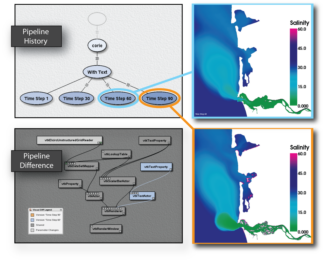
\includegraphics{VTKTextbook-38}\\
		\caption*{\texttt{The VisTrails multi-view visualization system.
				VisTrials enables interactive creation of visualization pipelines, maintaining the history of their evolution, optimizing their execution and allowing multiple pipelines to be compared in a spreadsheet-style layout.
				Image courtesy of SCI Institute University of Utah.}}
	\end{minipage}
\end{figure}

\firstletter{I}n the previous chapter we created graphical images using simple mathematical models for lighting, viewing, and geometry.
The lighting model included ambient, diffuse, and specular effects.
Viewing included the effects of perspective and projection.
Geometry was defined as a static collection of graphics primitives such as points and polygons.
In order to describe the process of visualization we need to extend our understanding of geometry to include more complex forms.
We will see that the visualization process transforms data into graphics primitives.
This chapter examines the process of data transformation and develops a model of data flow for visualization systems.

\section {Overview}
Visualization transforms data into images that efficiently and accurately convey information about
the data. Thus, visualization addresses the issues of transformation and representation.
